\section{Auswertung}

\begin{frame}{Auswertung}
	\begin{center}
		\begin{figure}[h]
			\begin{subfigure}[b]{0.45\textwidth}
				\centering
				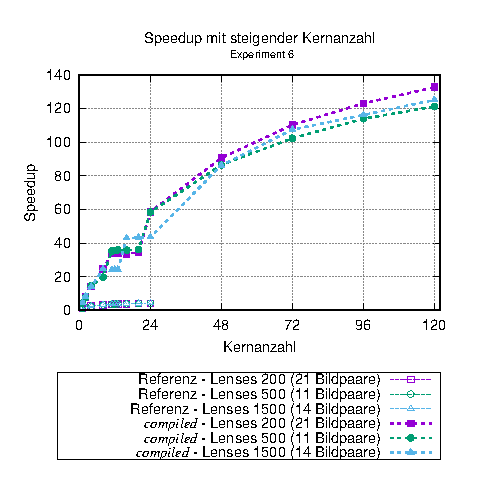
\includegraphics[width=\textwidth]{pdf/best_speedup_exp6}
				\caption{Experiment 6}
			\end{subfigure}
			\hfill
			\begin{subfigure}[b]{0.45\textwidth}
				\centering
				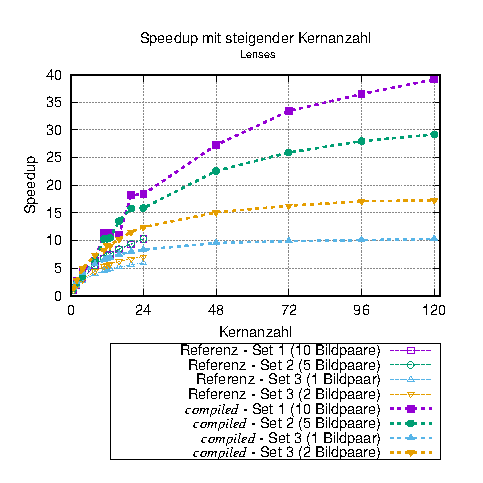
\includegraphics[width=\textwidth]{pdf/best_speedup_lenses}
				\caption{Lenses}
			\end{subfigure}
			\caption{Speed-Up \textit{compiled} gegenüber Referenz}
		\end{figure}
	\end{center}
\end{frame}

\begin{frame}{Auswertung}
	\textbf{Speed-Up:}
	\begin{itemize}
		\item Lenses Set 1: bis zu 40
		\item Experiment 6 Lenses 200: bis zu 130
	\end{itemize}
	$ \Rightarrow $ Echtzeitfähigkeit mit < 100 Taurus-Knoten nicht möglich
\end{frame}

\begin{frame}{Verbesserungsmöglichkeiten}
	\begin{itemize}
		\item Nutzen von FFTW
		\item Nutzen von GPGPUs
		\item Implementieren eines Belastungsausgleich
		\item Algorithmische Verbesserungen
	\end{itemize}
\end{frame}